% Source: Weinberg GR, physical PDF p. 471 (printed p. 448).
% Coverage: Figure 14.12, red shift versus corrected magnitude.
% Status: source plot extracted at source resolution; source-reviewed and compile-clean.
% Uncertainties: none.

\begingroup
\renewcommand{\thefigure}{14.12}
\begin{figure}[htbp]
  \centering
  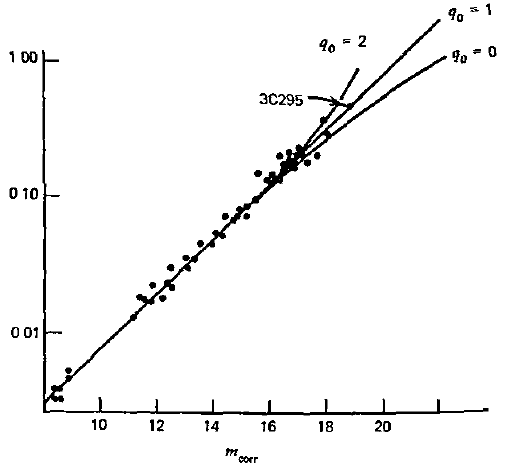
\includegraphics[width=0.64\textwidth]{figures/chapter14/fig14-12.png}
  \caption{Red shifts and corrected apparent magnitudes for 42 first-ranked
  cluster galaxies. Data are taken from a 1970 review of
  Sandage.\hyperref[ch14-ref-44]{\textsuperscript{44}} Curves represent fits
  of Eq.~\eqref{eq:14.6.10} to the data.}
  \label{fig:14.12}
\end{figure}
\endgroup
